\begin{center}
\begin{tikzpicture}
	\node[anchor=south west,inner sep=0] (image)  at (0,0) {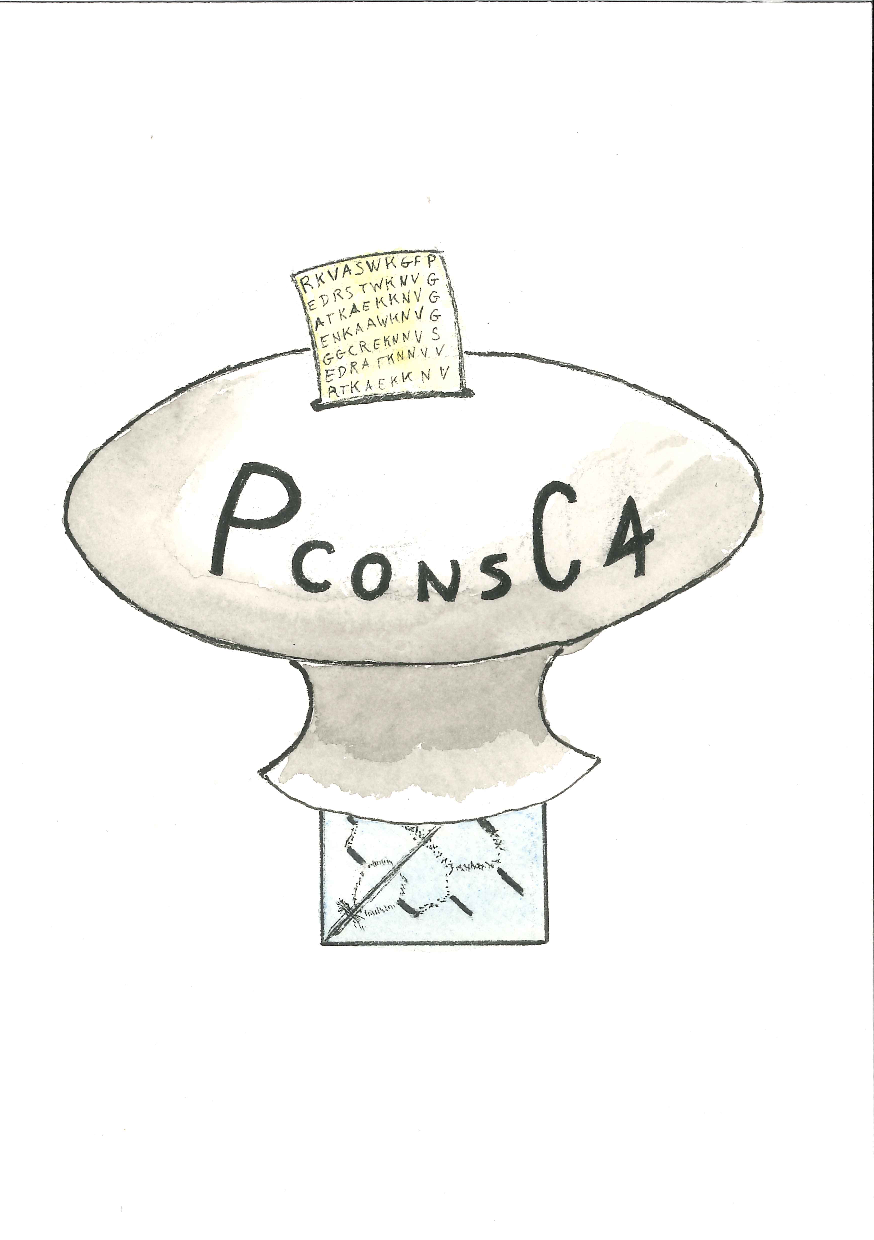
\includegraphics[trim={2mm, 2mm, 2mm, 2mm}, width=0.995\pagewidth]{scans/panel-3.pdf}};
    \begin{scope}[x={(current page.south east)},y={(current page.north west)}]
		\if\helplines1
			\draw[help lines,xstep=.1,ystep=.1] (0,0) grid (\N, \N);
		\else
			\path[help lines,xstep=.1,ystep=.1] (0,0) grid (\N, \N);
		\fi
			\node[align=center, text width=0.9\pagewidth](a) at (0.5, 0.92)  {\english{This paper presents PconsC4: a contact predictor for the future, that only requires one single alignment, and no external programs. }};
		
			\node[anchor=north](b) at (0.5, 0.15) {\english{It is 244 times faster, and yet, 12\% more accurate.}};
			
		    \node[align=center, text width=0.9\pagewidth, align=center, below=2mm of a] {\spanish{Este artículo presenta PconsC4: un predictor de contactos para el futuro, que sólo necesita un alineamiento, y ningún programa externo.}};
			\node[anchor=north, below=3mm of b]  {\spanish{Es \oldstylenums{244} veces más rápido, y aún así, \oldstylenums{12\%} más preciso.}};
				
    \end{scope}

\end{tikzpicture}
\end{center}
